% File example.tex
% Contact: simonnet@ecole.ensicaen.fr
%
% version 1.0 (July 24, 2009)
% version 1.1 (September 3, 2009)
% add using of the optional command: \secondauthoraddr



\documentclass[10pt]{article}

% File icdp2009.sty
% Preamble that you have to include to use the template  

% July 24, 2009
% Contact: simonnet@ecole.ensicaen.fr


\usepackage[a4paper,textwidth=18cm,textheight=24cm,top=2.85cm, bottom=2.85cm, left=1.5cm, right=1.5cm]{geometry}

\usepackage{template/icdp2009}

% left justified caption
\makeatletter
\long\def\@makecaption#1#2{%
\vskip\abovecaptionskip
\sbox\@tempboxa{#1. #2}%
\ifdim \wd\@tempboxa >\hsize
#1. #2\par
\else
\global \@minipagefalse
\hb@xt@\hsize{\box\@tempboxa\hfil}%
\fi
\vskip\belowcaptionskip}
\makeatother




%other package
\usepackage{amsmath}

% vectorial font
\usepackage{lmodern}

\usepackage{graphicx}
\usepackage{times}


\begin{document}
\noindent

\bibliographystyle{plain}

\title{Neural Networks\\Assignment 4 of Machine Learning I, 2021/2022}

\authorname{Mura Alessio}
\authoraddr{DIBRIS - Dipartimento di Informatica, Bioingegneria, Robotica e Ingegneria dei Sistemi\\
Università Degli Studi di Genova}

% \secondauthoraddr{+Affiliation,Country and contact details }


\maketitle

% % \keywords
% % Maximum 5 keywords placed before the abstract.

% \abstract
% This is where the abstract should be placed. It should consist
% of one paragraph and a concise summary of the material
% discussed in the article below. It is preferable not to use
% footnotes in the abstract or the title. The acknowledgement
% for funding organisations etc. is placed in a separate section at
% the end of the text. We wish you success with the preparation
% of your manuscript.

\section{Introduction}
Neural Networks are a set of simple algorithm that
are able to recognize patterns. Their name (and also structure) is inspired by the human brain.
\\\\
Neural Networks are commonly used in many applications,
e.g. prediction of stock market, weather forecasting and image
recognition. When a person tries to unlock his own phone
using his face, for example, almost always the smartphone
implements a neural network to recognize the allowed face
and unlock the phone.

\section{Theory of Neural Networks}
\subsection{Mathematical theory}
Neural network is made of \textit{neurons}. A neuron is a single
base unit that takes an input, computes a decision and gives
an output. The neuron can receive inputs either from outside
the neural network or from another neuron, and can also send
his output to the outside of the neural network of to another
neuron.
\\\\
Each neuron based his computation on a set of parameters
\textbf{w} called \textit{weights}, that slightly changes during all the learning
process. The \textit{weight update} (this is the name of the procedure)
follows this formula:
\begin{equation}
    \textbf{w}_l_+_1 = \textbf{w}_l + \Delta \textbf{w}_l
\end{equation}
Let \textbf{x} be the inputs of the neural network. The net input \textit{r}
can be defined as:
\begin{equation}
    r = \textbf{w} \cdot \textbf{x} = \sum_{i=1}^{d}{w_i x_i}
\end{equation}

Let \textit{a} be the \textit{activation value}, i.e. the output of the neuron. \textit{a} is computed as follows:
\begin{equation}
     a = f(r - \theta)
\end{equation}
where \textit{r} is the net input, $\theta$ is a threshold (an additional
weight) and \textit{f()} is the activation function. In particular, \textit{f()} can
correspond to many functions, e.g. \textit{Heaviside step, sigmoid,
hyperbolic tangent or softplus}.
\\\\\\\\\\
The correction factor $\Delta \textbf{w}_l$, used in formula 1, can then be
computed as:
\begin{equation}
     \Delta \textbf{w}_l = \eta \delta_l \textbf{x}_l
\end{equation}
where $\eta$ is a parameter and $\delta_l = \frac{1}{2}\left(t_l - a_l \right)$ (\textit{t} is the target of $x_l$).

\subsection{Multiple-layers Neural Network}
When there are more the one set of neurons operating at
the same \textit{depth}, then the neural network has \textit{multiple layers}.
The simplest multi-layer NN is a neural network which has
one input layer, one \textit{hidden layer} and one \textit{output layer}.
\\\\
The input layer takes \textbf{x} and spreads it to the \textit{hidden layer}.
The \textit{hidden layer} takes data from the \textit{input layer} and spreads
his calculations to the \textit{output} one, that gives the data to the
outside.
\\\\
The \textit{hidden layer} is called in this way because it is not
visible by the outside of the neural network. The more hidden
layers there are, the better the classification is. However,
many \textit{hidden layers} means many more computational power
required, so it is important to find the correct balance between
\textit{performance} and \textit{layers number}.
\subsection{Autoencoder}
An \textit{autoencoder} is a type of neural network. It has two main
features:
\begin{itemize}
 \item an \textit{autoencoder} has the same amount of output units
between input and output layers, while the hidden layer has
less neurons;
 \item the \textit{autoencoder} is trained using the same pattern as both
the input and the target, so that it is required to replicate the
input as output.
 \end{itemize} 
 The most important thing about an \textit{autoencoder} then are
the values of the hidden layer, because observations from the
same class will results in very similar weight \textbf{w}. At first sight
the \textit{autoencoder} can be seen as a \textit{classifier}. However this is
not the case, because it does not receive any \textit{target}, so it is
just unable to \textit{classify} something.

\section{THE ASSIGNMENT}
The given assignment consist of three tasks:
\begin{itemize}
 \item \textbf{Task 1}: Neural networks in Matlab
 \item \textbf{Task 2}: Feedforward multi-layer networks (multi-layer perceptrons)
 \item \textbf{Task 3}: Autoencoder
 \end{itemize} 

\subsection{Task 1: Neural networks in Matlab}
The first task simply ask to follow a tutorial for dealing with
Neural Networks in Matlab. For this purpose, it is require to
install and run the \textit{Deep Learning Toolbox}. The toolbox can be executed using the command \textit{nftool}, which toggle the toolbox
interface. 
\\\\
In order to solve an input-output problem, it is required to
load a data set. The toolbox provided some examples taken
from the UCI \textit{Machine Learning Repository}. For this example,
the body fat set is used. The sample are then divided in three
different subsets:
\begin{itemize}
 \item \textit{training subset} (70\% of the entire set);

 \item \textit{validation subset} (15\% of the entire set);
 \item \textit{test subset} (15\% of the entire set).
 \end{itemize} 
 Note that \textit{validation} set is useful to validate that the network
is generalizing and to stop training before overfitting (i.e. the
NN is trained \textit{too well}). With the overfitting, the network is
well trained on recognizing what he has already seen, but may
struggle on recognizing data that he has never seen.
\\\\
The toolbox then train a neural network and examine the
result, giving the possibility of plotting the regression, the
performance, the training state and the error histogram.

\subsection{Feedforward multi-layer networks}
The second task asks again to follow a tutorial. In this case
it is required to solve a patter recognition problem using a
two-layer feed-forward network. In particular, the hidden layer
has a \textit{sigmoid} transfer function, while the output layer has a
\textit{softmax} transfer function.
\\\\
Also in this case the set is divided in three subsets (with
the same percentage as before, 70\%,15\%,15\%). For this tasks,
two example sets were used, \textit{glass} set and \textit{iris} set.
\\\\
After selecting the set, in the toolbox (which can be executed using the command \textit{nprtool}) it is possible to select the
amount of \textit{hidden neurons}, i.e. the number of neurons of the
\textit{hidden layer} (default is 10).
\\\\
When the number of hidden neurons is defined, the toolbox
creates and trains a neural network with the given input set.
After the NN execution the toolbox is capable of plotting
the confusion matrices and the ROC (Receiving Operating
Characteristic).

\subsection{Autoencoder}
The third task asks to implement an \textit{autoencoder} in Matlab.
The used set is the MNIST set already used in Assignment 3,
and is made of 60.000 handwritten digit (from 0 to 9) stored
in a 28x28px grayscale images.
\\\\
From the MNIST set, it is required to extract only two
classes (i.e. digits) at the time, and give them as a unique
input set to the autoencoder. Since the set is quite large, from
the two class sets a fixed amount of observation are randomly
extracted (default is 250 per class set), in order to speed up
the execution.
\\\\
The two selected classes however are not random. For
this task, with the purpose of highlighting the autoencoder
performance, some pair of digits are quite easy to discern, while others may be much more difficult. The pair of classes
are:
\begin{equation}
    \textit{classes} =\begin{bmatrix}
            1&\textit{and}&6\\
            3 &\textit{and} &8\\
            1& \textit{and}& 7\\
            5& \textit{and} &6\\
        \end{bmatrix}
\end{equation}
An autoencoder can be initialized and trained in Matlab
using the functions \textit{trainAutoencoder()} and \textit{encode()}.\\
\textit{trainAutoencoder()} requires as inputs the data set and the
number of hidden nodes. For this simulation, in order to have
some viewable data, the number of hidden nodes has been set
to 2. Note that the \textit{Deep Learning Toolbox} uses a different
notation as in Machine Learning I course, so it is necessary to
transpose all the data before continuing. The function returns
an \textit{autoencoder variable}.
\\\\
\textit{encode()} is then used to encode the data, so that they are
ready to be plotted. \textit{encode()} requires two inputs, which are
the \textit{autoencoder} and the data set. It returns the encoded data.
\\\\
Finally the program plots the output of the two \textit{hidden neurons}, one per axes. The data are plotted using the \textit{plotcl()}
function, provided into the Machine Learning I course. The
function plots the data using different shapes and colours, that
corresponds to the class which the observation belongs to.
\\\\
If the two sets of different shapes and colours are distant
from each other, it means that the autoencoder has learned
well. Otherwise if the two sets are mixed, it means that the
learn process were more confused, and the two class aren’t
indistinguishable.
\newpage
\section{RESULTS}
Since task 1 and task 2 are two tutorials with their respective explanation, in this section we will focus on task 3 which requires us to implement an \textit{autoencoder}.

\begin{figure}[h] 
	\centering
	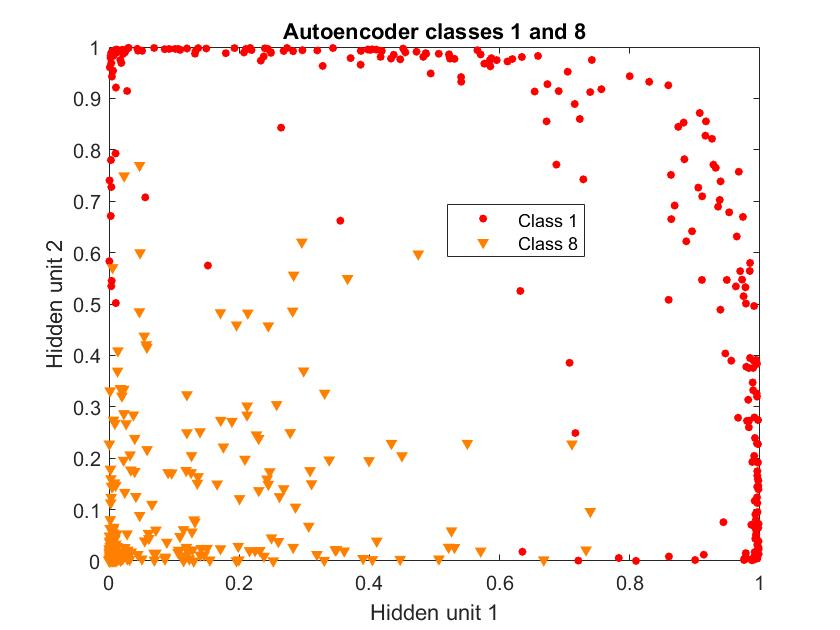
\includegraphics[width=0.9\columnwidth]{auto1.jpg} % Example image
	\caption{Autoencoder with classes 1 and 8.}
\end{figure}
In the figure 1 are represented the performance when the
input is made by observations belonging to class 1 (orange
triangles) and 8 (red dots). The two classes are generally
speaking very distant from each other (apart two red
dots that are very close to the class 1 region, meaning that an 8
is very similar to a 1), meaning that the two classes are quite
easily distinguishable.

\begin{figure}[h] 
	\centering
	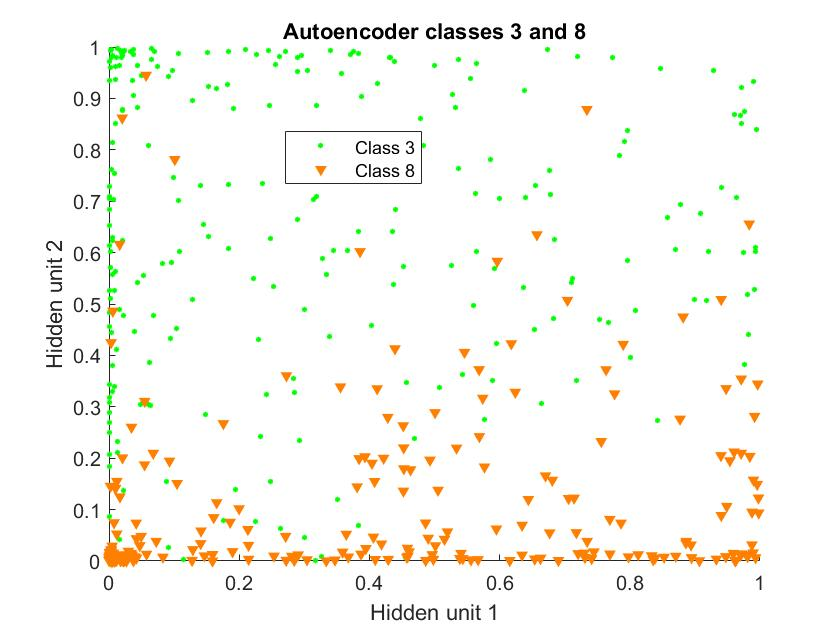
\includegraphics[width=0.9\columnwidth]{auto2.jpg} % Example image
	\caption{Autoencoder with classes 3 and 8.}
\end{figure}
The figure 2 produces a different output than the previous
one. At this time the autoencoder had to deal with different observations of the digits 3 (orange triangles) and 8 (green dots),
which can be very similar in many cases. The figure clearly
shows that the two digits are not easily distinguishable, and it
is highlighted by the fact that there are many threes inside the
top-left region (populated by eights), and the middle region of
the graph shows that many images can’t be understood easily.
\\
\begin{figure}[h] 
	\centering
	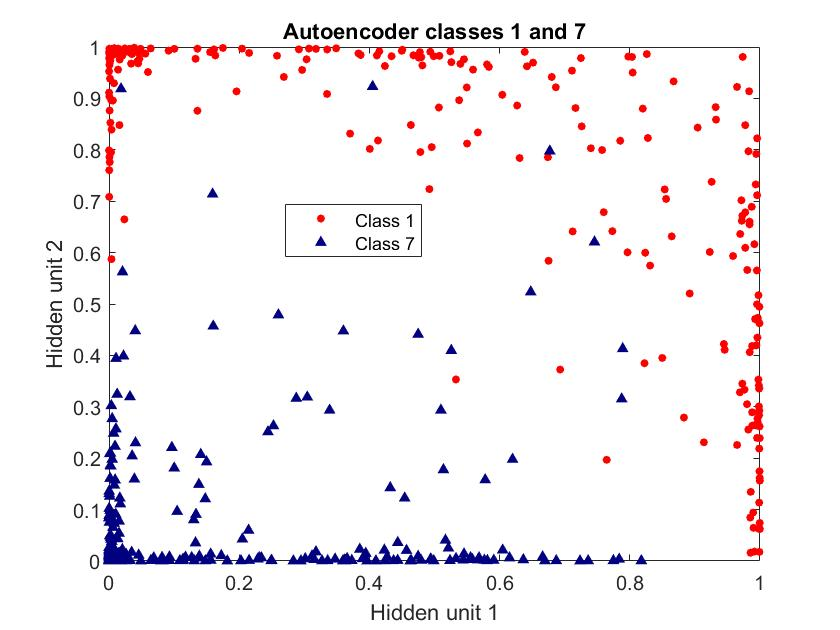
\includegraphics[width=0.9\columnwidth]{auto3.jpg} % Example image
	\caption{Autoencoder with classes 1 and 7.}
\end{figure}
\\\\
The figure 3 shows the outputs of the hidden neurons when the input correspond to a set of 1 (red dots) and 7 (blue
triangles). Also in this case there are some seven that are
interpreted as one and vice-versa. However, the data appears more ordered than before, meaning that the difference between
3 and 8 is less then the difference between 1 and 7.

\begin{figure}[h] 
	\centering
	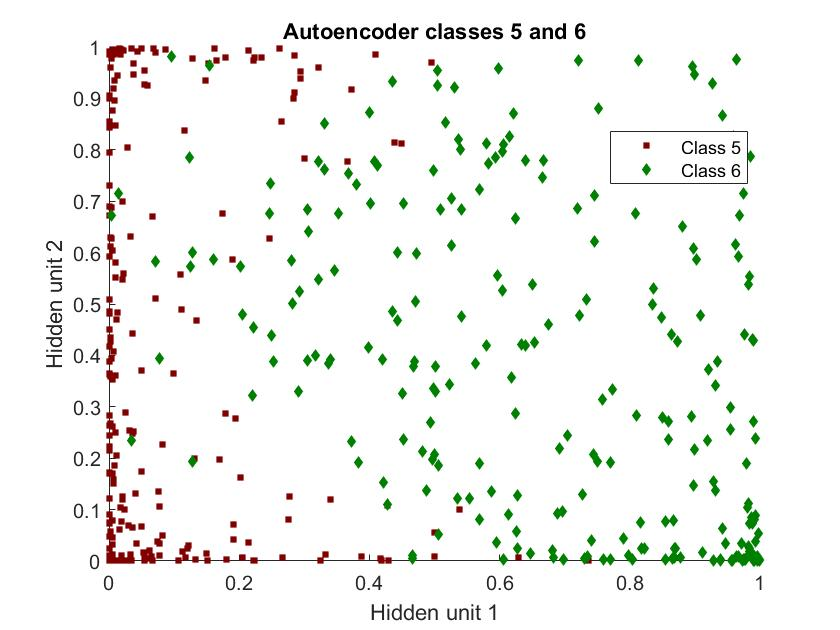
\includegraphics[width=0.9\columnwidth]{auto4.jpg} % Example image
	\caption{Autoencoder with classes 5 and 6.}
\end{figure}
The figure 4 shows the results of a set made by observations belonging to classes 5 (dark red squares) and 6
(green diamonds). Here we can see something different than
in previous cases, because many images representing the 6
seems to be similar to images that represents 5, but not viceversa. Generally speaking, this could mean that some 6 are
similar to 5, but almost ever a 5 is distinguishable from a 6.

\end{document}